% Document class and parameters %
\documentclass[10pt,a4paper]{article}

% Document packages %
\usepackage{graphicx}
\usepackage{biblatex}
\usepackage{parskip}
\usepackage{listings}
\usepackage{caption}
\usepackage{subcaption}
\usepackage{amsmath}
\usepackage[most]{tcolorbox}


\graphicspath{{./Images/}}
\setlength{\parskip}{1em}

% Document Body %
\begin{document}
\begin{titlepage}
	\centering
	{\scshape\LARGE Imperial College London \par}
	\vspace{1cm}
	{\scshape\Large Mathematics: Year 2\par}
	\vspace{1.5cm}
	{\huge\bfseries Random variables and Distributions \par}
	\vspace{2cm}
	{\Large\ Xin Wang }
	\vfill
	{\large \today\par}
\end{titlepage}

\begin{abstract}
    A probability distribution is the mathematical function that gives the probabilities of
    occurrence \textbf{of all the different possible outcomes for an experiment}. This is similar to
   a graph giving a visual picture of the function i.e. it is a visual mathematical
    description of a random phenomenon in terms of its sample space and the probabilities of events.
\end{abstract}

\tableofcontents
\pagebreak

%%%%%%%%%%%%%%%%%%%%%%%%%%%%%%%%%%%%%%%%%%%%%%%%%%%%%%%%%%%%%%%%%%%%%%%%%%%%%%%%%%%%%%%%%%%%%%%%%%%%%%%%%%
\section{Notations}

The probability of the random variable $X$ taking on a specific value $x$ is denoted as $$X = x$$
\begin{itemize}
    \item \textbf{Uppercase letters}: Random variables
    \item \textbf{Lowercase letters}: Particular values a random variable can take on
\end{itemize}

The probability function:
$$
    P(X=x)
$$
interpreted as "the probability that the random variable $X$ takes the value $x$".
%%%%%%%%%%%%%%%%%%%%%%%%%%%%%%%%%%%%%%%%%%%%%%%%%%%%%%%%%%%%%%%%%%%%%%%%%%%%%%%%%%%%%%%%%%%%%%%%%%%%%%%%%%
\section{Random Variables}

Random variables are a variable in which its values depends on outcome of a random phenomenon.

\begin{tcolorbox}[breakable,colback=white]
\textbf{Random variable} $X$ (on a sample space $S$):  A measurable function that assigns a
real numbered value to each outcome of $S$.
\\
\\
\textbf{Range} (of a random variable): The collection of values a random variable can take on.
\end{tcolorbox}


The \textbf{range} of the random variables determines whether it is a:
\begin{itemize}
    \item \textbf{Discrete random variable}: A random variable that can take on values in a specified
    countable list e.g. coin toss or dice roll.

    Has a \textbf{probability mass function} that is characteristic of the random variable's probability distribution.
    \item \textbf{Continuous random variable}: A random variable that can take on \textbf{any}
    numerical value \textbf{in an interval}.

    Has a \textbf{probability density function} that is characteristic of the random variable's probability distribution.
\end{itemize}

\pagebreak
%%%%%%%%%%%%%%%%%%%%%%%%%%%%%%%%%%%%%%%%%%%%%%%%%%%%%%%%%%%%%%%%%%%%%%%%%%%%%%%%%%%%%%%%%%%%%%%%%%%%%%%%%%
\section{Probability distribution functions}

Often a sample space can be very large and general. By using probability distributions of a specific random
variable, focus can be directed to a specific range in order to simplify the description and
analysis of a random experiment. Probability theory becomes more useful in practice.

\begin{tcolorbox}[breakable,colback=white]
\textbf{Probability distribution}: A list of all of the possible outcomes of a random variable along with their corresponding probability values.
\end{tcolorbox}

\begin{figure} [h!]
    \centering
    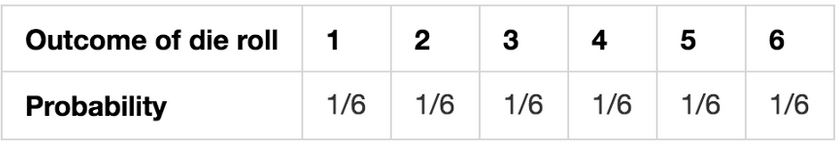
\includegraphics[scale=0.4]{Prob distribution.JPG}
    \caption{An example of a discrete probability distribution}
\end{figure}

In many scenarios, the number of outcomes can be much larger or infinite and a table would be
impractical to write. To get around the problem of writing a table for every distribution, a
function is defined. \textbf{A function gives the ability to define a probability distribution succinctly}.

As mentioned previously, a function is fundamentally is a box that \textbf{takes an input} and
\textbf{returns an output}. The main benefit of functions is the knowledge of how to transform
any input into the output, this knowledge can be used to visualise the function explicitly as a
graph.

One of the most important features of functions are \textbf{parameters}. Parameters are the most
important feature of a probability distribution function because, fundamentally, they define the
final output of the function i.e. the likelihood of certain outcomes in a random process. It’s often
parameters that statisticians try to estimate in data science problems. 

\begin{tcolorbox}[breakable,colback=white]
    \textbf{Probability distribution function}: A function that defines a particular probability
    distribution e.g. CDF, PDF and PMF.
\end{tcolorbox}

%%%%%%%%%%%%%%%%%%%%%%%%%%%%%%%%%%%%%%%%%%%%%%%%%%%%%%%%%%%%%%%%%%%%%%%%%%%%%%%%%%%%%%%%%%%%%%%%%%%%%%%%%%
\subsection{Cumulative distribution function}

The cumulative distribution function (CDF) of a random variable is a method to describe the
distribution of random variables. The advantage of the CDF is that it can be defined for any kind of
random variable e.g. discrete, continuous and mixed.

\begin{tcolorbox}[breakable,colback=white]
\textbf{Cumulative Distribution Function (CDF)} $F(x)$: The probability that a random variable $X$ taking a value \textbf{less than} or \textbf{equal to} $x$.
$$
    F_X(x) = P(X \leq x) \; \text{for all } x\in \Re 
$$
\end{tcolorbox}

\textbf{Example 1}: The probability that the random variable has value less than 3 $\{X \leq 3\}$ is
an union of probabilities $\{X=0\}$, $\{X=1\}$, $\{X=2\}$ and $\{X=3\}$.
\begin{align*}
    P(X\leq 3) &= P(X=0) + P(X=1) + P(X=2) + P(X=3) \\
    &= 0.6561 + 0.2916 + 0.0486 + 0.0036 \\
    &= 0.9999
\end{align*}

And $P(X=3)$ can be found with:
\begin{align*}
    P(X=3) &= P(X\leq 3) - P(X\leq 2) \\
    &= 0.0036
\end{align*}
    
Note: the CDF completely describes the distribution of a discrete random variable. The CDF can also be used to derive the PMF.

\textbf{Example 2}: Determine the PMF of $x$ from the following CDF:
$$
    F(x) = 
    \begin{cases}
        0 & x < -2 \\ 
        0.2 & -2\leq x < 0 \\
        0.7 & 0 \leq x < 2 \\
        1 & 2\leq x
    \end{cases}
$$

\begin{figure} [h!]
    \centering
    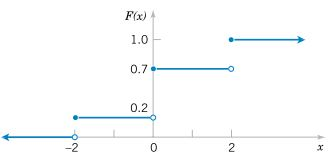
\includegraphics[]{Ex2_1.JPG}
    \caption{The Cumulative Distribution Function}
\end{figure}

\textbf{The PMF at each point is the change in the CMF at that point}:
\begin{align*}
    f(-2) &= 0.2 - 0 = 0.2 \\
    f(0) &= 0.7 - 0.2 = 0.5 \\
    f(2) &= 1.0 - 0.7 = 0.3
\end{align*}

\textbf{Example 1}: Suppose $X_1 \sim \text{Unif}(0,1)$ and $X_2 \sim \text{Unif}(0,1)$ ,and $X_1$
and $X_2$ are independent.

Compute the probability that $P(X_1\leq \frac{1}{2} \cap X_2 \leq \frac{1}{2})$.
\begin{enumerate}
    \item Use the CDF:
    \begin{align*}
        P\left(X_i \leq \frac{1}{2}\right) = F_X\left(\frac{1}{2}\right) = \frac{1}{2}
    \end{align*}
    \item Note that $X_1$ and $X_2$ are independent:
    \begin{align*}
        P\left(X_1 \leq \frac{1}{2} \cap X_2 \leq \frac{1}{2}\right) &= F_X\left(\frac{1}{2}\right)F_X\left(\frac{1}{2}\right) \\
        &= \frac{1}{4}
    \end{align*}
\end{enumerate}

\pagebreak


\textbf{Example 3}: Time until chemical reaction is approximated by the continuous CDF:
$$
    F(x) = 
    \begin{cases}
        0 & x<0 \\
        0.01e^{-0.01x} & 0 \leq x   
    \end{cases}
$$
Find the PDF of $X$ and what is the proportion of reactions is completed \textbf{within} 200
milliseconds?
\begin{enumerate}
    \item Find the PDF:
    \begin{align*}
        f(x) = 
        \begin{cases}
            0 & x < 0 \\
            0.01e^{-0.01x} & 0 \leq x    
        \end{cases}
    \end{align*}
    \item Probability that reactions complete within 200 milliseconds:
    \begin{align*}
        P(X<200) = F(200) = 1 - e^{-2} = 0.8647
    \end{align*}
\end{enumerate}

When trying evaluate the probabilities of the form $P(a < X \leq b)$:
\begin{align*}
    P(a<X\leq b) &= P(X\leq b) - P(X \leq a) \\
    &= F_X(b) - F_X(a) \\
    &= \int_a^b f_X(x) \: dx
\end{align*}

If $b$ is close enough to $a$:
\begin{align*}
    P(a<X\leq b) &= F_X(b) - F_X(a) \\
    &= \int_a^b f_X(x)\: dx \\
    &\approx f_X(a)(b-a)
\end{align*}

\pagebreak

%%%%%%%%%%%%%%%%%%%%%%%%%%%%%%%%%%%%%%%%%%%%%%%%%%%%%%%%%%%%%%%%%%%%%%%%%%%%%%%%%%%%%%%%%%%%%%%%%%%%%%%%%%
\subsection{Theoretical Mean and Variance}

As mentioned previously, parameters are very important in functions and two of the most important
parameters when it comes to probability distributions are: \textbf{mean} and \textbf{variance}.

\begin{tcolorbox}[breakable,colback=white]
    \textbf{Expectation operator} $E$: The computation that finds the sum of function
    $X$ that is weighted by the corresponding probability.
\end{tcolorbox}

These parameters are often used to summarise a probability distribution of a random variable $X$.
Note that these two numbers \textbf{do not uniquely define a distribution}, some distributions could
have the same mean and variance.
\begin{itemize}
    \item \textbf{Mean}: A measure of the center of the probability distribution.
    \item \textbf{Variance}: A measure of the dispersion i.e. variability in the distribution.
\end{itemize}

\begin{tcolorbox}[breakable,colback=white]
\textbf{Mean} or \textbf{Theoretical mean} $E(X)$ or $\mu$: Weighted average of the possible values
of $X$ where the weights are defined as the probabilities.
$$
    \mu = E(X) = \sum_x x\:f(x)
$$
or 
$$
    \mu = E(X) = \int_{-\infty}^{\infty}x f(x) \: dx
$$
\end{tcolorbox}

If $f(x)$ is thought of as a probability mass function of a loading on a long, thin beam, $E(X)$ is the
point at which the beam balances. This reiterates the definition that $E(X)$ describes the center of the
distribution of $X$.

Properties:
\begin{itemize}
    \item $E(aX+b)=aE(X)+b$ for any $a,b \in \Re$
    \item $E[g(X)]=\sum_x g(x)f_X(x)$ for any function $g(x)$
\end{itemize}

\begin{figure} [h!]
    \centering
    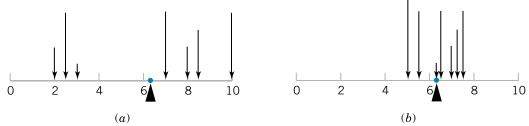
\includegraphics[]{Mean.JPG}
    \caption{PMF with triangle representing the graphical representation of Mean}
\end{figure}

\pagebreak

\begin{tcolorbox}[breakable,colback=white]
    \textbf{Variance} or \textbf{Theoretical variance} $\sigma^2$ or $V(X)$: A measure of the dispersion
    or the scatter of the distribution.
    $$
        E(X-\mu)^2 = \sum_x(x-\mu)^2f(x) = \sum_xx^2f(x)-\mu^2
    $$
    or
    $$
       E(X^2) - E(X)^2
    $$
    where $V(X) \geq 0$
    \\
    \\
    \textbf{Standard deviation} $\sigma$: A measure of how much the members of a group
    differ \textbf{relative from the mean value $\mu$}.
    $$
        \sigma = \sqrt{\sigma^2}
    $$
\end{tcolorbox}

Some distributions may have the same mean but different variances. 

\begin{figure} [h!]
    \centering
    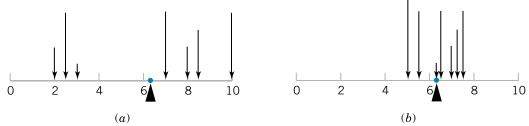
\includegraphics[]{Mean.JPG}
    \caption{PMF $(a)$ and $(b)$ showing different variance but same mean}
\end{figure}

Properties:
\begin{itemize}
    \item $V(aX+b)=a^2V(X)$ for any $a,b \in \Re$
\end{itemize}

\textbf{Example 1}: Given the discrete random variable $Y$ with range $[1,2,\dots,5]$ with the
following probability distribution, find the variance and standard deviation.
\begin{figure} [h!]
    \centering
    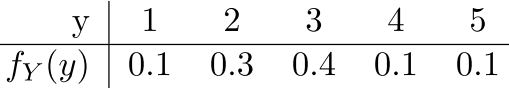
\includegraphics[scale=0.4]{ex2.JPG}
\end{figure}
\begin{enumerate}
    \item Find the Mean $\mu$:
    \begin{align*}
        \mu &= E(Y) \\
        &= 1(0.1) + 2(0.3) + 3(0.4) + 4(0.1) + 5(0.1) \\
        &= 2.8
    \end{align*}

    \item Find the variance:
    \begin{align*}
        V(Y) &= \sum_y (y-\mu)^2f_Y(y) \\
        &= (1-2.8)^2(0.1)+(2-2.8)^2(0.3)+(3-2.8)^2(0.4)+(4-2.8)^2(0.1)+(5-2.8)^2(0.1) \\
        &= 1.16
    \end{align*}

    \item Standard deviation:
    \begin{align*}
        \sigma &= \sqrt{1.16} \\
        &\approx 1.8
    \end{align*}
\end{enumerate}

\textbf{Example 2}: Given the following:
$$
    f_X(x) = 
    \begin{cases}
        cx^2 & 0 \leq x \leq 2 \\
        0 & \text{Otherwise}    
    \end{cases}
$$
\begin{enumerate}
    \item Find the value of $c$ for which $f_X$ is a \textbf{valid density}.
        \begin{align*}
            \int_{-\infty}^\infty f_X(x)\: dx &= 1 \\
        \end{align*}
        Thus:
        \begin{align*}
            \int_0^2 cx^2 \: dx &= \left[\frac{cx^3}{3}\right]_0^2 \\
            &= \left(\frac{8}{3}\right)c \\
        \end{align*}
        Simplifying to:
        \begin{align*}
            \frac{8}{3}c &= 1 \\
            c &= \frac{3}{8}
        \end{align*}
    \item Obtain the CDF.
    \begin{align*}
        F_X(u) &= \int_0^u \frac{3}{8}x^2 \: dx \\
        &= \frac{3}{8} \int x^2\: dx \\
        &= \frac{3}{8}\left[\frac{x^3}{3}\right]_0^u \\
        &= \frac{u^3}{8}
    \end{align*}
    CDF is:
    \begin{align*}
        F_X(u) = 
        \begin{cases}
            0 & u<0 \\
            \frac{u^3}{8} & 0\leq u \leq 2 \\
            1 & u>2
        \end{cases}
    \end{align*}
    \item Compute $P(1<X \leq 2)$.
    \begin{align*}
        P(1 < X \leq 2) &= F_X(2) - F_X(1) \\
        &= \frac{2^3}{8}-\frac{1^3}{8} \\
        &= \frac{7}{8}
    \end{align*}
\end{enumerate}

%%%%%%%%%%%%%%%%%%%%%%%%%%%%%%%%%%%%%%%%%%%%%%%%%%%%%%%%%%%%%%%%%%%%%%%%%%%%%%%%%%%%%%%%%%%%%%%%%%%%%%%%%%
\subsection{Probability mass function}

When a probability function is used to describe a discrete probability distribution, it is called a
\textbf{probability mass function (PMF)}.

A PMF $f$ returns the probability of an outcome $x$. Therefore, a probability mass function is written
as:
\begin{align*}
    f(x) = P(X=x)
\end{align*}
\begin{center}
    \textit{probability mass function $f$ just returns the probability of the outcome $x$}
\end{center}

Since the PMF returns probabilities, it must obey the axioms of probability that described
previously: \par 
\begin{itemize}
    \item The PMF outputs values between $0$ and $1$ inclusive.
    $$
        0 \leq f(x) \leq 1
    $$
    \item The sum of the PMF over all outcomes is equal to $1$.
    $$
        \sum_i f(x_i) = f(x_1) + f(x_2) + \dots = 1
    $$
\end{itemize} 
A discrete probability distribution can be described as a \textbf{table}, as a \textbf{function}
and, also, graphically. \par
\begin{figure} [h!]
    \centering
    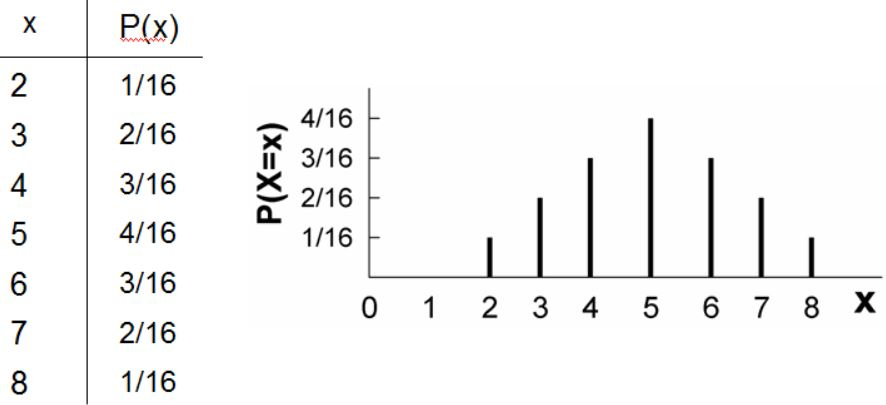
\includegraphics[scale=0.4]{PMF table.JPG}
    \caption{Graphically representing a discrete probability distribution}
\end{figure}
Some probability distributions crop up so often that they have been extensively studied and have
names. This will be covered in later chapters.
\begin{itemize}
    \item \textbf{Bernoulli distribution} $\text{Ber}(p)$: Models an experiment with only two possible outcomes.
    \item \textbf{Binomial distribution} $\text{Bin}(n,p)$: Models the number of successes when someone draws $n$ times with replacement.
    \item \textbf{Geometric distribution} $\text{Geo}(p)$: Models the number of trials needed to get one success.
    \item \textbf{Poisson distribution} $\text{Pois}(\lambda)$: Models the probability of a given number of events occurring in a fixed interval of time or space if these events occur with a known constant mean rate and independently of the time since the last event.
\end{itemize}

%%%%%%%%%%%%%%%%%%%%%%%%%%%%%%%%%%%%%%%%%%%%%%%%%%%%%%%%%%%%%%%%%%%%%%%%%%%%%%%%%%%%%%%%%%%%%%%%%%%%%%%%%%
\subsection{Probability density function}

Some probabilities of random variables have continuous outcomes e.g. the height of an adult picked
at random from a population or the amount of time that a taxi driver has to wait before their next
job. For these examples, the random variable is better described by a continuous probability
distribution.

When a probability function is used to describe a continuous probability distribution, it is called
a \textbf{probability density function (PDF)}. Probability density functions are slightly more
complicated conceptually. 
\begin{align*}
    P(X\leq x_0) = F_X (x_0) = \int_{-\infty}^{x_0} f_X (x)\: dx
\end{align*}

where $F_X$ is monotonically non-decreasing i.e. $F_X(a) \leq F_X(b)$ if $a<b$ ,and $F_X(-\infty)=0$
and $F_X(\infty)=1$
\begin{align*}
    P(a<X\leq b) = P(X\leq b)-P(X\leq a) = F_X(b)-F_X(a) = \int_a^b f_X(x) \: dx
\end{align*}
where if $b$ is close enough to $a$ then
\begin{align*}
    P(a<X\leq b) = F_X(b)-F_X(a) = \int_a^b f_X(x)\: dx \approx f_X(a)(b-a)
\end{align*}

%%%%%%%%%%%%%%%%%%%%%%%%%%%%%%%%%%%%%%%%%%%%%%%%%%%%%%%%%%%%%%%%%%%%%%%%%%%%%%%%%%%%%%%%%%%%%%%%%%%%%%%%%%
\subsubsection{Properties of continuous probability distribution}

\begin{enumerate}
    \item Numbers on the vertical axis start at zero and go up. Any output value from a probability
    density function is \textbf{greater than or equal to zero} i.e. the output is non-negative:
    \begin{align*}
        f(x) \geq 0
    \end{align*}
    \item Unlike probability mass functions, the output of a probability density function \textbf{is
    not a probability value}. The probability between two outcomes, $a$ and $b$ is the integral of the probability density function between those two points which is equivalent to finding the area under the curve produced by the probability density function between the points $a$ and $b$:
    \begin{align*}
        \int_a^b f(x;\: \mu, \sigma) dx = P(a<X<b)
    \end{align*}
    \begin{center}
        \textit{the integral of the probability density function between 'b' and 'a' (left-hand side) is equal to the probability that the outcome of the random variable is between a and b (right-hand side)}
    \end{center}
    \item Remember that rules of probability distributions still apply, namely that the sum of all possible outcomes is equal to $1$:
    \begin{align*}
        \int_{-\infty}^\infty f(x) dx = 1
    \end{align*}
    \item The probability of the random variable being equal \textbf{to a specific outcome} is $0$.
    For example, the probability that the outcome is equal to the number $2$ is defined as:
    \begin{align*}
        \int^2_2 f(x)dx = P(2<X<2) = 0
    \end{align*}
    Problems only deal with: 
    \begin{itemize}
        \item Probabilities occurring between two values.
        \item Probability of an outcome being greater than or less than a specific value.
    \end{itemize}
\end{enumerate}

\textbf{Example 1}: Given 
$$f_X(x)=\begin{cases}
    cx^2 & 0\leq x\leq 2 \\
    0 & \text{Otherwise} 
\end{cases}$$
\begin{itemize}
    \item Find value of $c$ for which $f_X$ is a valid density:
    
    Require:
    \begin{align*}
        \int_{-\infty}^{\infty} f_X(x)\: dx &= 1 
    \end{align*}
    Thus:
    \begin{align*}
        \int_0^2 cx^2 \: dx &= \left[\frac{cx^3}{3}\right]_0^2 = \left(\frac{8}{3}\right)c = 1 \\
        c &= \frac{3}{8}
    \end{align*}
    \item Obtain CDF:
    
    For $0\leq x \leq 2$, the CDF is:
    \begin{align*}
        F_X(u)=\int_0^u \frac{3}{8}x^2 \: dx = \frac{3}{8} \int x^2 \: dx = \frac{3}{8}\left[\frac{x^3}{3}\right]_0^u = \frac{u^3}{8}
    \end{align*}
    The CDF is:
    \begin{align*}
        F_X(u) = \begin{cases}
            0 & u<0 \\
            \frac{u^3}{8} & 0\leq u \leq 2 \\
            1 & u>2
        \end{cases}
    \end{align*}
    \item Compute $P(1< X \leq 2)$:
    \begin{align*}
        P(1<X\leq 2) = F_X(2)-F_X(1) = \frac{2^3}{8}-\frac{1^3}{8} = \frac{7}{8}
    \end{align*}
\end{itemize} 

%%%%%%%%%%%%%%%%%%%%%%%%%%%%%%%%%%%%%%%%%%%%%%%%%%%%%%%%%%%%%%%%%%%%%%%%%%%%%%%%%%%%%%%%%%%%%%%%%%%%%%%%%%
\section{Discrete Probability Distributions}
%%%%%%%%%%%%%%%%%%%%%%%%%%%%%%%%%%%%%%%%%%%%%%%%%%%%%%%%%%%%%%%%%%%%%%%%%%%%%%%%%%%%%%%%%%%%%%%%%%%%%%%%%%
\subsection{Discrete uniform distribution: $X \sim \text{Unif}(a,b)$}

The simplest discrete random variable where one assumes \textbf{only a finite number of possible values},
each with equal probability. A simple example of the discrete uniform distribution is throwing a fair die. The possible values are $1, 2, 3, 4, 5, 6$ and each time the die is thrown the probability of a given score is $\frac{1}{6}$.

\begin{tcolorbox}[breakable,colback=white]
\textbf{Discrete uniform distribution}: The distribution of a random variable where each of its $n$ values
within the range have equal probability:
$$
    f(x_i) = \frac{1}{n}
$$
\end{tcolorbox}

Common properties:
\begin{itemize} 
    \item Probability mass unction:
    $$
        f_X(x) = \frac{1}{k} \; \text{for}\; x = 1,2,\dots,k
    $$
    Equally distributed with even spacing.

    \item Cumulative distribution function: 
    $$
        F_X (x) = \sum_{i=1}^x \frac{1}{k} = \frac{x}{k} \; \text{for}\; x=1,2,\dots,k
    $$
    \item Mean:
    \begin{align*}
        E(X) = \frac{k+1}{2} \; \text{where}\; k \text{ is the number of elements in the distribution} 
    \end{align*}

    \item Variance:
    \begin{align*}
        V(X) = E(X^2)-E(X)^2 = \frac{k^2 - 1}{12}
    \end{align*}
\end{itemize}

\begin{figure} [h]
\centering
\begin{subfigure}{.5\textwidth}
  \centering
  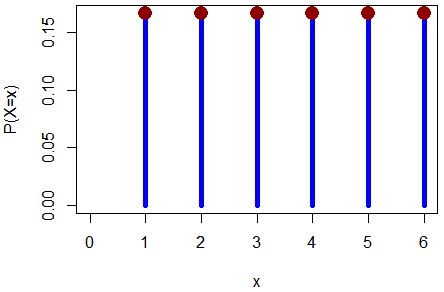
\includegraphics[scale=0.52]{Uniform discrete.JPG}
  \caption{Probability mass function}
\end{subfigure}%
\begin{subfigure}{.5\textwidth}
  \centering
  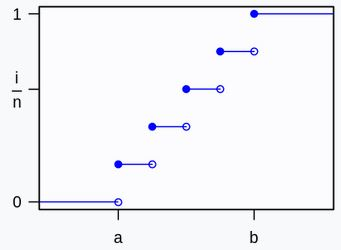
\includegraphics[scale=0.6]{Uniform discrete CDF.JPG}
  \caption{Cumulative distributive function}
\end{subfigure}
\end{figure}

\pagebreak

%%%%%%%%%%%%%%%%%%%%%%%%%%%%%%%%%%%%%%%%%%%%%%%%%%%%%%%%%%%%%%%%%%%%%%%%%%%%%%%%%%%%%%%%%%%%%%%%%%%%%%%%%%
\subsection{Bernoulli distribution: $X\sim \text{Be}(p)$}

The Bernoulli distribution is the \textbf{discrete probability distribution} of a random variable
which takes a binary, boolean output:
\begin{itemize}
    \item $1$ with probability $p$
    \item $0$ with probability $1-p$
\end{itemize} 

\begin{tcolorbox}[breakable,colback=white]
    \textbf{Bernoulli trails}: Independent trails with a constant probability $p$ of a success on each trail.
\end{tcolorbox}

Key characteristics of a bernoulli trail:
\begin{itemize}
    \item Only two possible outcomes e.g. H or T
    \item $n$ identical trails
    \item Trails are \textbf{independent} - one event does not affect the other event
    \item Constant probability of success $p$ 
\end{itemize}

The probability function associated with a Bernoulli variable is the following:
\begin{figure} [h!]
    \centering
    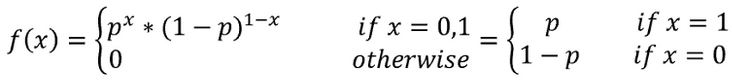
\includegraphics[scale=0.6]{Bernoulli.JPG}
\end{figure}
\begin{itemize}
    \item Expected Value:
    \begin{align*}
        E(X) = p
    \end{align*}
    \item Variance:
    \begin{align*}
        V(X) = p(1-p)
    \end{align*} 
\end{itemize}

\begin{figure} [h!]
    \centering
    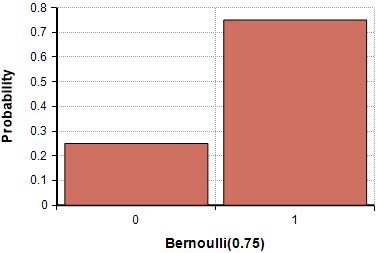
\includegraphics[scale=0.7]{Bernoulli distribution.JPG}
    \caption{Example of Bernoulli distribution}
\end{figure}


The idea behind the Bernoulli distribution is that the experiment is done \textbf{only once}. But
what happens if there is more than one trial, under the assumption that trials are independent
among each other?

\pagebreak

%%%%%%%%%%%%%%%%%%%%%%%%%%%%%%%%%%%%%%%%%%%%%%%%%%%%%%%%%%%%%%%%%%%%%%%%%%%%%%%%%%%%%%%%%%%%%%%%%%%%%%%%%%
\subsection{Binomial distribution: $X \sim \text{Bin}(n,p)$}

This distribution describes the behavior the outputs of n random experiments, each having a Bernoulli distribution with probability $p$.

Combinatorial notation defined as:
$$
    C(n,x) = {n\choose x}= \frac{n!}{x!(n-x)!}
$$
where:
\begin{itemize}
    \item $n$: Number of trails
    \item $x$: Number of successes
\end{itemize}

Running $n$ independent experiments with each having a Bernoulli distribution with parameter $p$,
the probability of having $x$ successes is defined:
\begin{align*}
    f(x) = 
    \begin{cases}
        {n \choose x} p^x \times (1-p)^{n-x} & \text{if } x = 0,1,\dots,n \\ 
        0 & \text{Otherwise}
    \end{cases}
\end{align*}

\begin{itemize}
    \item Expected Value:
    \begin{align*}
        E(X) = np
    \end{align*}
    \item Variance: 
    \begin{align*}
         V(X) = np(1-p)
    \end{align*}
\end{itemize}

\textbf{Example 1}: A fair coin is tossed $6$ times with sample space $S=\{H,T\}$. Note this is a
binomial experiment with $n=6$ and $p=q=\frac{1}{2}$.
\begin{enumerate}
    \item Probability of exactly two H: $x = 2$ and $n-x = 4$:
    \begin{align*}
        f_X(2;n=6,p=\frac{1}{2})&={6\choose 2} \left(\frac{1}{2}\right)^4 \left(\frac{1}{2}\right)^2 \\
        &= \frac{6!}{2!(6-2)!} \left(\frac{1}{4}\right) \left(\frac{1}{16}\right) \\
        &\approx 0.23
    \end{align*}

    \item $E$ denotes event where \textbf{at least} 4 H is achieved i.e. 4, 5 and 6 H's, find the probability.
    \begin{align*}
        P(E) &= \sum_{x\in\{4,5,6\}} f_X\left(x; n=6, p=\frac{1}{2}\right) \\
        &= {6\choose 4}\left(\frac{1}{2}\right)^4\left(\frac{1}{2}\right)^2 + {6\choose 5}\left(\frac{1}{2}\right)^5\left(\frac{1}{2}\right) + {6\choose 6}\left(\frac{1}{2}\right)^6\left(\frac{1}{2}\right)^0 \\
        &= \frac{15}{64} + \frac{6}{64} + \frac{1}{64}\\
        &= \frac{11}{32} \\
        &\approx 0.34
    \end{align*}

    \item Find the probability of getting no heads i.e. all failures:
    \begin{align*}
        (1-6)^6 &= \left(\frac{1}{2}\right)^6 \\
        &= \frac{1}{64}
    \end{align*}
\end{enumerate}

%%%%%%%%%%%%%%%%%%%%%%%%%%%%%%%%%%%%%%%%%%%%%%%%%%%%%%%%%%%%%%%%%%%%%%%%%%%%%%%%%%%%%%%%%%%%%%%%%%%%%%%%%%
\subsection{Geometric distribution: $X\sim \text{Geom} (p)$}

The idea of Geometric distribution is modeling the probability of having a certain number of
Bernoulli trials (each with parameter $p$) before getting the first success. The random variable $X$
denotes the number of trails until first success.

Computing the probability of having first $k-1$ failures, each with probability $1-p$, and then, at
the $k$th trial, having a success (with probability $p$). Since each Bernoulli trial is independent
from the others:
\begin{align*}
    f(x) = (1 - p)^{x-1}\times p 
\end{align*}
\begin{itemize}
    \item Mean: 
    \begin{align*}
        E(X) = \frac{1}{p}
    \end{align*}
    \item Variance: 
    \begin{align*}
        V(X) = \frac{(1-p)}{p^2}
    \end{align*}
\end{itemize}

\textbf{Example 1}: Let random variable $X$ denote the number of bits transmitted up till and
including the first error. The probability that a bit transmitted through a channel has an error is
$0.1$ (Probability of a successful transmission is $0.9$). 

Find the probability that the 5th bit is an error:
\begin{align*}
    P(X=5) &= P(OOOOE) \\
    &= 0.9^4 \times 0.1 \\
    &= 0.066
\end{align*}

\pagebreak
\begin{figure} [h!]
    \centering
    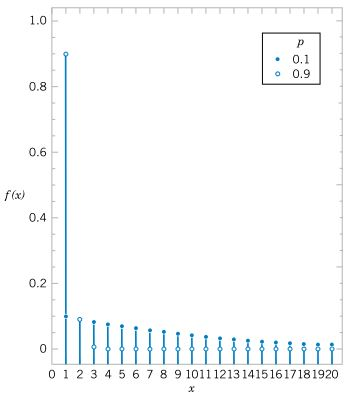
\includegraphics[scale=.8]{GeoDis.JPG}
\end{figure}

Note how the probability of an error bit (0.1) and successful bit (0.9) gradually converge as the
value of $x$ increases.

%%%%%%%%%%%%%%%%%%%%%%%%%%%%%%%%%%%%%%%%%%%%%%%%%%%%%%%%%%%%%%%%%%%%%%%%%%%%%%%%%%%%%%%%%%%%%%%%%%%%%%%%%%
\subsection{Poisson distribution: $X \sim \text{Po}(\lambda)$}

A \textbf{Poisson Process} is a model for a series of discrete event where the \textbf{average time
between events is known, but the exact timing of events is random}. Many physical problems are
concerned with events occurring independently of any medium such as time and space e.g. number of
aircraft accidents in a set time or counts measured by a Geiger-counter in an certain time interval.

A Poisson Process meets the following criteria:
\begin{enumerate}
    \item Events are independent of each other. The occurrence of one event does not affect the
    probability another event will occur (waiting time between events is memoryless).
    \item The average rate $\lambda$ (events per time period) is constant.
    \item Two events cannot occur at the same time.
\end{enumerate}

The Poisson distribution gives the probability of observing $k$ events in a time period given the
length of the period and the average events per time: \par
\begin{align*}
    P(k\text{ events in time period}) = e^{-\left(\frac{\text{events}}{\text{time}}\times \text{time period}\right)} \times \frac{\left(\frac{\text{events}}{\text{time}}\times \text{time period}\right)^k}{k!}
\end{align*}
$\frac{\text{events}}{\text{time}} \times \text{time period}$ is usually simplified into \textbf{the
rate parameter}: lambda $\lambda$.
\begin{align*}
    P(k\text{ events in time period}) = e^{-\lambda} \times \frac{\lambda^k}{k!}
\end{align*}

\begin{itemize}
    \item Mean: 
    \begin{align*}
        E(X) = \lambda
    \end{align*}
    \item Variance: 
    \begin{align*}
        V(X) = \frac{(1-p)}{p^2}
    \end{align*}
\end{itemize}

Lambda can be thought of as the expected number of events in the interval. As we change the rate
parameter $\lambda$ the probability of seeing different numbers of events in one interval changes.

\begin{figure} [h!]
    \centering
    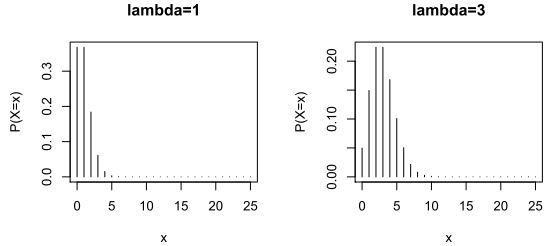
\includegraphics[scale=0.85]{PMF poisson.JPG}
    \caption{PMF for poisson distributions for selected value of $\lambda$}
\end{figure}

When calculating probabilities, means and variances, it is important to \textbf{use consistent
units} i.e. if average number of flaws \textbf{per millimeter} is $3.4$ then average number of flaws
in \textbf{10 millimeter} is 34.

\textbf{Example 1}: Suppose accidents occur following a Poisson distribution at a \textbf{rate of 2
per year}.
\begin{enumerate}
    \item What is the probability of \textbf{more than one accident} in a six-month period?
        \begin{enumerate}
            \item Let $X$ denote the number of accidents in a six month period:
            $$
                X \sim \text{Poisson}\left(2\;.\;\frac{1}{2}\right)
            $$
            \item Establish the cases:
            $$
            f_X{x;\lambda = 1} = 
            \begin{cases}
                \frac{e^{-1}1^x}{x!} & x = 0,1,2,\dots \\
                0 & \text{Otherwise}    
            \end{cases}
            $$
            \item Find the probability that \textbf{only one} accident occur and subtract from 1:
            \begin{align*}
                P(X>1;\lambda = 1) &= 1 - P(X\leq 1; \lambda = 1) \\
                &= 1 - \left\{f_X(0; \lambda = 1)+f_X(1;\lambda = 1)\right\} \\
                &= 1 - \left\{\frac{e^{-1}}{0!}+\frac{e^{-1}}{1!}\right\} \\
                &= 1 -2e^{-1} \\
                &\approx 0.264
            \end{align*}
        \end{enumerate}
    \item What is the probability of \textbf{at least two accidents} \textbf{in a one year period}?
        \begin{enumerate}
            \item Let $Y$ denote the number of accidents in a year:
            $$
                Y \sim \text{Poisson}\left(2\right)
            $$
            \item Establish the cases:
            $$
            f_Y{y} = 
            \begin{cases}
                \frac{e^{-2}2^y}{y!} & y = 0,1,2,\dots \\
                0 & \text{Otherwise}    
            \end{cases}
            $$
            \item Find the probability that \textbf{only one} accident occur and subtract from 1:
            \begin{align*}
                P(Y>1;\lambda = 2) &= 1 - P(Y\leq 1; \lambda = 2) \\
                &= 1 - \left\{f_Y(0; \lambda = 2)+f_Y(1;\lambda = 2)\right\} \\
                &= 1 - \left\{\frac{e^{-2}}{0!}+\frac{e^{-2}\times 2}{1!}\right\} \\
                &= 1 -3e^{-2} \\
                &\approx 0.594
            \end{align*}
        \end{enumerate}
\end{enumerate}

\textbf{Example 2}: Births in a hospital occur randomly at an average rate of 1.8 births per hour.
What is the probability of observing \textbf{4 births in a given hour} at the hospital?
\begin{enumerate}
    \item Let $X = \text{Number of births in a given hour}$:
    \begin{align*}
        \text{Mean rate } \lambda = 1.8 \\
        \Rightarrow X \sim \text{Po}(1.8)
    \end{align*}
    \item Use the formula to calculate the probability of observing exactly 4 births in a given hour:
    \begin{align*}
        P(X=4) = e^{-1.8}\frac{1.8^4}{4!} = 0.0723 
    \end{align*}
\end{enumerate}

\pagebreak

%%%%%%%%%%%%%%%%%%%%%%%%%%%%%%%%%%%%%%%%%%%%%%%%%%%%%%%%%%%%%%%%%%%%%%%%%%%%%%%%%%%%%%%%%%%%%%%%%%%%%%%%%%
\section{Continuous Probability Distributions}

A continuous distribution displays the \textbf{ranges of probabilities for the outcomes of a random
variable with infinite values} and is used to model a continuous random variable. Continuous
distributions has a range of values that are infinite, and therefore uncountable. For example, time
is infinite since one could count from $0$ seconds to a billion, a trillion and so on. 

\begin{tcolorbox}[breakable,colback=white]
\textbf{Continuous probability distribution}: A probability distribution where the random variable
$X$ can take on any value i.e. continuous.
\end{tcolorbox}

Recall that probability is defined as $\frac{\text{Desired outcome}}{\text{Number of possible
outcomes}}$ e.g. a fortune wheel divided into $20$ sectors resulting in a probability of
$\frac{1}{20}$ of landing in any section. Imagine the fortune is then partitioned into an infinite number of
sectors of equal area but each of those would have an area of $0$. Due to the infinite nature and
the definition of probability mentioned above, the \textbf{probability of a continuous random
variable taking on any one specific value is $0$}. 

But remember the total probability must be $1$ in order to satisfy one of the axioms of probability:
\begin{align*}
    P(-\infty \leq X \leq \infty) = \int_{-\infty}^{\infty}f(x)\: dx = 1
\end{align*} 
which creates an apparent contradiction. That is why when working with continuous distributions,
probabilities are only assigned to an interval. The probability that $X$ falls between two values
($a$ and $b$) equals the integral (area under the curve) from $a$ to $b$.

As mentioned previously with its infinite range, a continuous probability distribution cannot be
expressed in tabular form like discrete probability distribution. Instead, an equation or formula is
used to describe a continuous probability distribution i.e. \textbf{probability density function}.

The probability density function satisfies several condition properties:
\begin{itemize}
    \item The random variable $Y$ is a function of $X$ i.e. $y = f(x)$
    \item The value of $y$ is greater than or equal to zero for all values of $x$
    \item The total area under the curve of the function is equal to $1$
\end{itemize}

\pagebreak

%%%%%%%%%%%%%%%%%%%%%%%%%%%%%%%%%%%%%%%%%%%%%%%%%%%%%%%%%%%%%%%%%%%%%%%%%%%%%%%%%%%%%%%%%%%%%%%%%%%%%%%%%%
\subsection{Continuous uniform distribution: $X \sim \text{Unif}(a,b)$}

The uniform distribution for continuous random variables is one of the simplest distribution. In a
uniform distribution, all possible values of a continuous random variable inside some interval have
the same probability. 

Since all values of such random variable inside an interval have the same probabilities, the
probability density function is defined as:
\begin{align*}
    f_X(x) = 
    \begin{cases}
        \frac{1}{b-a} & a \leq x \leq b \\
        0 & \text{Otherwise}    
    \end{cases}
\end{align*}
\begin{itemize}
    \item Cumulative distribution function:
    \begin{align*}
        F_X(u) = 
        \begin{cases}
            0 & u < a \\
            \int_a^u \frac{1}{b-a} \: dx = \frac{u-a}{b-a} & a\leq u\leq b \\
            1 & u > b
        \end{cases}
    \end{align*}
    \item Mean $\mu$:
    \begin{align*}
        \mu = E(X) = \frac{(a+b)}{2}
    \end{align*}
    \item Variance $\sigma^2$:
    \begin{align*}
        \sigma^2 = V(X) = \frac{(b-a)^2}{12}
    \end{align*}
\end{itemize}

%%%%%%%%%%%%%%%%%%%%%%%%%%%%%%%%%%%%%%%%%%%%%%%%%%%%%%%%%%%%%%%%%%%%%%%%%%%%%%%%%%%%%%%%%%%%%%%%%%%%%%%%%%
\subsection{Exponential distribution: $X \sim \text{Exp}(\lambda)$}

The exponential distribution is the probability distribution of the \textbf{time between events} in a Poisson
point process i.e. a process in which events occur continuously and independently at a constant
average rate $\lambda$. Exponential distribution and Poisson distribution is closely related. It can
be considered the continuous analogue of the geometric distribution and it has the key property of
being \textbf{memoryless}. 

Commonly used to model the lifetime of electronic components. Previously mentioned Poisson
distribution defined a random variable as the number of flaws along a length of copper wire. The
\textbf{distance between the flaws} is another random variable of interest. 

For example, let random variable $X$ denote the length from any starting point on the wire until a flaw is found.
The distribution of $X$ (distance between flaws) can be obtained from knowledge of the distribution
of the number of flaws. 

In general if random variable $N$ is defined as the number of flaws in $x$ millimeters of wire and
$\lambda$ (per unit measurement) is defined as the mean number of flaws, $N$ has a Poisson distribution
with \textbf{mean} of $\lambda x$:
\begin{align*}
    P(X>x) &= P(N=0) \\
    &= \frac{e^{-\lambda x}(\lambda x)^0}{0!} \\
    &= e^{-\lambda x}
\end{align*}

Common assumption that the wire is longer than the value of $x$ and the $x$ is non-negative $x > 0$.

The CDF of function $X$ is:
\begin{align*}
    F(x) = P(X\leq x) = 1 - e^{-\lambda x} 
\end{align*}
The PDF of function $X$ is:
\begin{align*}
    f(x) = \lambda e^{-\lambda x}
\end{align*}
\begin{itemize}
    \item Mean: $\mu = E(X) = \frac{1}{\lambda}$ 
    \item Variance: $\sigma^2 = V(X) = \frac{1}{\lambda^2}$
\end{itemize}

To verify that the PDF is valid, note that the density must be non-negative:
\begin{align*}
    \int_{-\infty}^{\infty} f_X (x;\lambda)\: dx &= \int_0^{\infty} \lambda e^{-\lambda x} dx \\
    &= \left[-e^{-\lambda x}\right]_0^\infty \\
    &= [0-(-1)] \\
    &= 1
\end{align*}

The starting point for measuring $X$ does not matter because the probability of the number
of flaws in an intercal of a Poisson process depends on the length of the interval, not the starting
location.

\textbf{Example 1}: Given a computer network, user log-ins can be modeled as Poisson process with a
mean of 25 log-on \textbf{per hour} $(\mu = 25)$. What is the probability that there are no log-ins
in an interval of 6 minutes?

\begin{enumerate}
    \item Specify the interval investigated: 
    
    Let $X$ denote the \textbf{time in hours} from the start of the interval until the first log-in.
    \item Establish provided data: 
    
    $X$ has exponential distribution where $\lambda = 25$ log-in per hour.
    \item Convert into same units of measurement: 
    
    As we are interested in the probability that $X$ exceeds $6$ minutes, $6$ minutes in hours is $0.1$ hours.
    \item Extract data from PDF: 
    
    Note $\lambda = 25$ and $u = 0.1$
    \begin{align*}
        P(X>0.1) &= \int_{u}^{\infty} \lambda e^{-\lambda x}\: dx \\
        &= \int_{0.1}^{\infty} 25e^{-25 x} \: dx \\
        &= e^{-25(0.1)} \\
        &= 0.082
    \end{align*}
\end{enumerate}

%%%%%%%%%%%%%%%%%%%%%%%%%%%%%%%%%%%%%%%%%%%%%%%%%%%%%%%%%%%%%%%%%%%%%%%%%%%%%%%%%%%%%%%%%%%%%%%%%%%%%%%%%%
\subsubsection{Memoryless Property}

Exponential distribution has an important interesting property with conditional probability.

\textbf{Example 1}: Let $X$ denote the time between detections of a particle with a geiger counter
and $X$ has an exponential distribution with $\lambda = 1.4$ minutes. 
\begin{enumerate}
    \item The probability that a particle is detected within $30$ seconds ($0.5$ minute) of starting the counter:
    \begin{align*}
        P(X<0.5 \text{ minute}) &= F(0.5) \\
        &= 1 - e^{-\frac{0.5}{1.4}} \\
        &= 0.30
    \end{align*}

    \item If $3$ minutes has passed without a particle detected, what are the probability that a
    particle is detected in the next $30$ seconds?

    One might assume that the probability should be greater than $0.3$ but the nature of exponential
    distribution means that \textbf{it is not true, the probability will remain the same}. The
    conditional probability of the above scenario after $3$ minutes can be defined as:
    \begin{align*}
        P(X<3.5 | X>3) = \frac{P(3<X<3.5)}{P(X>3)}
    \end{align*}
    where $P(3<X<3.5)$ and $P(X>3)$ are defined as:
    \begin{itemize}
        \item $P(3<X<3.5)$: 
        \begin{align*}
            P(3<X<3.5) &= F(3.5) - F(3) \\
            &= \left[1 - e^-{\frac{3.5}{1.4}}\right] - \left[1 - e^-\frac{3}{1.4}\right] \\
            &= 0.0035
        \end{align*}
        \item $P(X>3)$: 
        \begin{align*}
            P(X>3) &= 1 - F(3) \\
            &= e^{-\frac{3}{1.4}} \\ 
            &= 0.117
        \end{align*}
    \end{itemize}

    therefore:
    \begin{align*}
        P(X<3.5 | X>3) = \frac{0.035}{0.117} = 0.30
    \end{align*}

    \item After $3$ minute without a detection, the probability of particle detection within the
    next $30$ seconds is the \textbf{same} probability of detection in the next $30$ seconds after starting.
\end{enumerate}

Only exponential distributions have this unique property:
\\
\begin{tcolorbox}[breakable,colback=white]
\textbf{Memoryless property}: For an exponential random variable $X$:
$$
    P(X<t_1 + t_2 | X>t_1) = P(X<t_2)
$$
\end{tcolorbox}

\begin{figure} [h!]
    \centering
    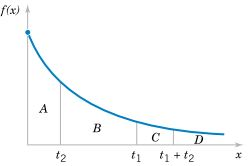
\includegraphics[]{Memoryless.JPG}
    \caption{Graphical representation of \textit{memoryless} property}
\end{figure}
The above figure shows that the proportion of the area of region $A$ divided by total area under the PDF ($A+B+C+D$)
is the same as the proportion fo region $C$ divided by the total area under the PDF ($C+D$). 

The property is intuitive since, with Poisson distributions, it is assumed that intervals can be
partitioned into small intervals that are \textbf{independent}. This is similar to Bernoulli trails
where the knowledge of previous process does not affect the probabilities of events in future
sub-intervals.

This type of modelling is seen in reliability studies of electronics for the time until device
failure. Due to the memoryless property, regardless of how long the device has been operating, the
probability of a failure in the next $x$ hours is the same in the first $x$ hours.

%%%%%%%%%%%%%%%%%%%%%%%%%%%%%%%%%%%%%%%%%%%%%%%%%%%%%%%%%%%%%%%%%%%%%%%%%%%%%%%%%%%%%%%%%%%%%%%%%%%%%%%%%%
\subsection{Normal distribution: $X \sim N(\mu,\: \sigma^2)$}

The normal distribution is the most common distribution in all of probability and statistics. One of the main reasons it crops up so much is due to the Central Limit Theorem.

Originally found by De Moivre called the Central Limit Theorem and also called the Gaussian
distribution. The most widely used model for the distribution of a random variable. Whenever a
random experiment is performed, the random variable corresponding to the average tends to have a
normal distribution. 

\begin{figure} [h!]
    \centering
    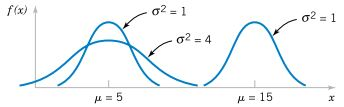
\includegraphics[]{Normalintro.JPG}
    \caption{Normal probability distribution with different values of the parameters $\mu$ and $\sigma^2$}
\end{figure}

\textbf{Normal random variable}: A random variable $X$ with probability density function:
$$
    f(x) = \frac{1}{\sqrt{2\pi}\times \sigma} e^{\frac{-(x-\mu)^2}{2\sigma^2}} \; \text{where:} -\infty < x < \infty
$$
with parameters $\mu$ where $-\infty < \mu < \infty$ and $\sigma$ where $\sigma > 0$.
\begin{itemize}
    \item $E(X) = \mu$ 
    \item $V(X) = \sigma^2$
\end{itemize}

\begin{figure} [h!]
    \centering
    \includegraphics[]{standardnormal.JPG}
    \caption{Standard normal distribution, note the symmetrical shape about $\mu$}
\end{figure}

\begin{tcolorbox}[breakable,colback=white]
    \textbf{Standard normal random variable} ($Z$): A normal random variable with $\mu=0$ and $\sigma^2
    = 1$
    \begin{enumerate}
        \item $\phi(z)$ - PDF of a standard normal random variable.  
        \begin{align*}
            \phi(z) = \frac{1}{\sqrt{2\pi}}e^{-\frac{z^2}{2}}
        \end{align*}
        \item $\Phi$ - CDF of a standard normal random variable.
        \begin{align*}
            \Phi(z) = \int_{-\infty}^z \phi(u)\: du
        \end{align*}
    \end{enumerate}
\end{tcolorbox}

A standard normal distribution has:
\begin{itemize}
    \item Mean $\mu$ of $0$
    \item Variance $\sigma^2$ of $1$
\end{itemize}

Change of variable techniques apply to normal distributions:

\textbf{Example 1}: If $Z\sim N(0,1)$ and $X=\sigma Z + \mu$ then find $X \sim N(\mu, \sigma^2)$.
\begin{align*}
    f_X(x) &= f_Z(z) \left| \frac{dz}{dx}\right| \\
    &= \phi \left(\frac{x - \mu}{\sigma}\right)\left| \frac{d}{dx} \frac{x-\mu}{\sigma} \right| \\
    &= \frac{1}{\sqrt{2\pi \sigma^2}}e^{-\frac{(x-\mu)^2}{2\sigma^2}}
\end{align*}

which is the PDF of $N(\mu,\: \sigma^2)$

%%%%%%%%%%%%%%%%%%%%%%%%%%%%%%%%%%%%%%%%%%%%%%%%%%%%%%%%%%%%%%%%%%%%%%%%%%%%%%%%%%%%%%%%%%%%%%%%%%%%%%%%%%
\subsubsection{Normal distribution table}

With normal distribution, the CDF cannot be obtained usually. Probability calculations have to be
used in conjunction with tables obtained through numeral integration such as:

\begin{figure} [h!]
    \centering
    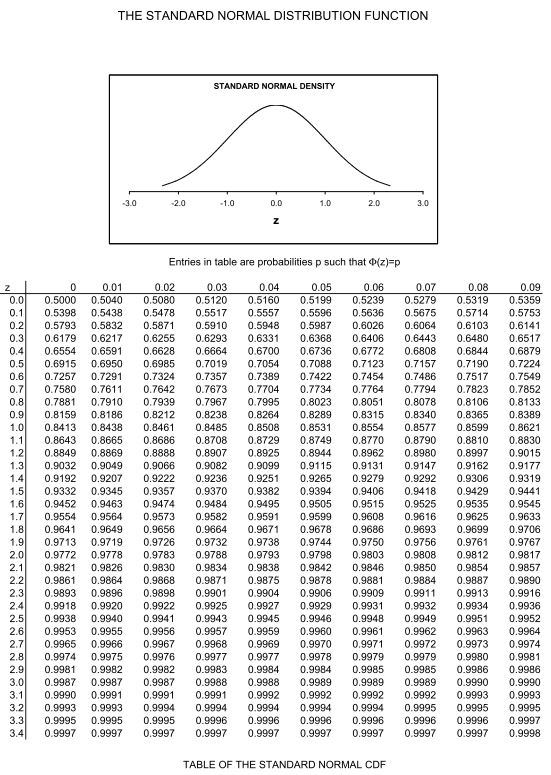
\includegraphics[scale=0.6]{Table.JPG}
\end{figure}

The table is a tabulation such that $\Phi(z)= p$ for $z \geq 0$.

\textbf{Example 1}: Find $P(Z \leq 1.6)$.
\begin{align*}
    P(Z\leq 1.6) = \Phi(1.6) = 0.9452
\end{align*} 
\begin{tcolorbox}[breakable,colback=white]
    For $z<0$, the symmetry of the standard normal distribution about its mean $\mu$ is exploited.
    \begin{align*}
        \Phi(z)+\Phi(-z) = 1 \\ 
        \Rightarrow \Phi(-z) = 1 - \Phi(z)
    \end{align*}
\end{tcolorbox}

\textbf{Example 2}: Find $P(Z \leq -0.75)$.
\begin{align*}
    P(Z \leq -0.75) &= 1 - \phi(0.75) \\
    &= 1 - 0.7734 \\
    &= 0.2266
\end{align*}
\textbf{Note}:
\begin{enumerate}
    \item The table is applicable to the first decimal place, any questions can be rounded to the nearest
    position.
    \item The $Z$ is concentrated between $-3$ and $3$ [Three-Sigma Rule].
\end{enumerate}

%%%%%%%%%%%%%%%%%%%%%%%%%%%%%%%%%%%%%%%%%%%%%%%%%%%%%%%%%%%%%%%%%%%%%%%%%%%%%%%%%%%%%%%%%%%%%%%%%%%%%%%%%%
\subsubsection{Standardising}

Since calculating probabilities of standard normal random variables requires a table, using the same
approach for any arbitrary normal random variable would need a specific separate table for every possible
pair of values for $\mu$ and $\sigma$. Alternatively, any normal distributions are related
algebraically and can be transformed into the standard normal random variable.

Any normal distribution can be transformed into a standard normal by:
\begin{enumerate}
    \item Subtracting the mean $\mu$ 
    \item Dividing by the standard deviation $\sigma$
\end{enumerate}
\begin{figure} [h!]
    \centering
    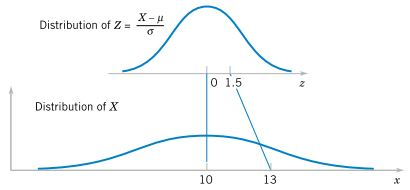
\includegraphics[scale=0.9]{Standard.JPG}
    \caption{Graphical representation of Standardising}
\end{figure}
\begin{align*}
    Z = \frac{X - \mu}{\sigma}
\end{align*}

The new variable $Z$ represents the distance of $X$ from its mean ($\mu$) in terms of standard
deviations ($\sigma$).

The \textbf{Three Sigma Rule} still applies and is defined as the following: X is concentrated
between $\mu - 3\sigma$ and $\mu + 3\sigma$.

\textbf{Example 1}: Given $X \sim N(3,\:5^2)$, standardise it and the following probabilities:
$P(X<5)$ and $P(0.5<X<5.5)$.
\begin{enumerate}
    \item Standardise the expression $X$:
    \begin{align*}
        Z = \frac{(X-3)}{5} \sim N(0,\: 1)
    \end{align*}

    \item Compute $P(X<5)$: 
    \begin{align*}
        P(X<5) &= P\left(\frac{X-3}{5}<\frac{5-3}{5}\right) \\
        &= P(Z<0.4) \\
        &= \Phi(0.4) \\
        &= 0.655
    \end{align*}

    \item Compute $P(0.5 < X < 5.5)$:
    \begin{align*}
        P(0.5 < X < 5.5) &= P\left(\frac{0.5-3}{5}<\frac{X-3}{5}<\frac{5.5-3}{5}\right) \\
        &= \Phi(0.5) - \Phi(-0.5) \\
        &= \Phi(0.5) - [1-\Phi(0.5)] \\ 
        &= 2\Phi(0.5) - 1 \\
        &= 2(0.6915) - 1 \\
        &= 0.3830
    \end{align*}
\end{enumerate}

%%%%%%%%%%%%%%%%%%%%%%%%%%%%%%%%%%%%%%%%%%%%%%%%%%%%%%%%%%%%%%%%%%%%%%%%%%%%%%%%%%%%%%%%%%%%%%%%%%%%%%%%%%
\subsection{Chi-squared distribution: $X \sim \chi^2(k)$}

The chi-square distribution with $k$ degrees of freedom is the distribution of a sum of the squares
of $k$ independent standard normal random variables. It is a special case of the gamma distribution
and is one of the most widely used probability distributions in inferential statistics.

\begin{figure} [h!]
    \centering
    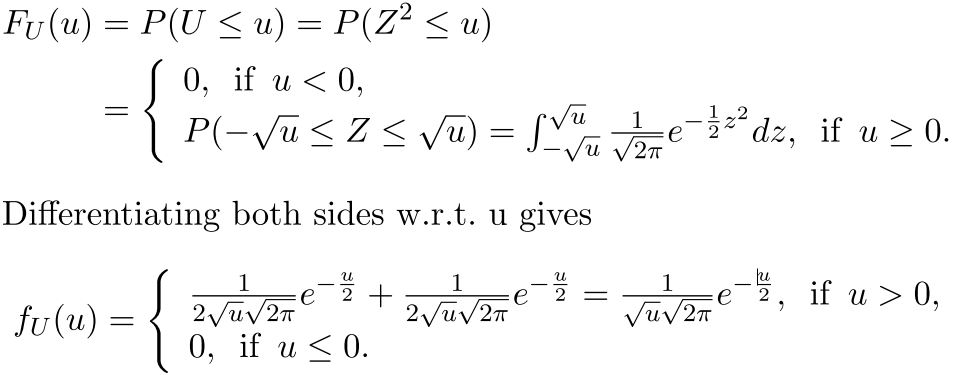
\includegraphics[scale=0.5]{Chi.JPG}
\end{figure}

%%%%%%%%%%%%%%%%%%%%%%%%%%%%%%%%%%%%%%%%%%%%%%%%%%%%%%%%%%%%%%%%%%%%%%%%%%%%%%%%%%%%%%%%%%%%%%%%%%%%%%%%%%
\subsection{Log-normal distribution: $X \sim \text{lognormal}(\mu, \sigma^2)$}

A log-normal distribution is a continuous probability distribution of a random variable whose
logarithm is normally distributed. Thus, if the random variable $X$ is log-normally distributed,
then $Y = ln(X)$ has a normal distribution. Equivalently, if $Y$ has a normal distribution, then the
exponential function of $Y, X = exp(Y)$ has a log-normal distribution. 

A random variable which is log-normally distributed takes only positive real values. It is a
convenient and useful model for measurements in exact and engineering sciences, as well as medicine,
economics and other topics e.g., energies, concentrations, lengths, financial returns and other metrics. 

\begin{figure} [h!]
    \centering
    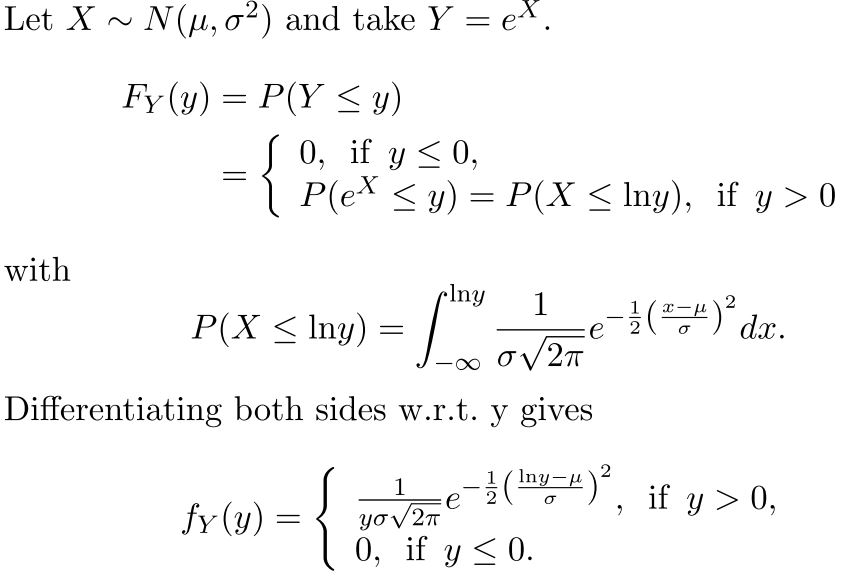
\includegraphics[scale=0.5]{Log.JPG}
\end{figure}

%%%%%%%%%%%%%%%%%%%%%%%%%%%%%%%%%%%%%%%%%%%%%%%%%%%%%%%%%%%%%%%%%%%%%%%%%%%%%%%%%%%%%%%%%%%%%%%%%%%%%%%%%%
\section{Change of Variable Technique}

If the probability density function of a random variable $X$ is given as $f_X(x)$, it is
possible to calculate the probability density function of some variable $Y = g(X)$.

There is a simple rule to compute the probability density function of the new random variable $Y$ in terms of
the probability density function of the original random variable $X$.

%%%%%%%%%%%%%%%%%%%%%%%%%%%%%%%%%%%%%%%%%%%%%%%%%%%%%%%%%%%%%%%%%%%%%%%%%%%%%%%%%%%%%%%%%%%%%%%%%%%%%%%%%%
\subsection{Generalisation for an increasing function}

Let:
\begin{itemize}
    \item $X$ be a \textbf{continuous random variable}.
    \item $g(x)$ a strictly monotonic function (one-to-one function) defined over the support $c_1 < x < c_2$.
    \item $Y = g(X)$ be a continuous and increasing function of $X$ with inverse function $X=g^{-1}(Y)$ 
\end{itemize} 

\begin{figure} [h!]
    \centering
    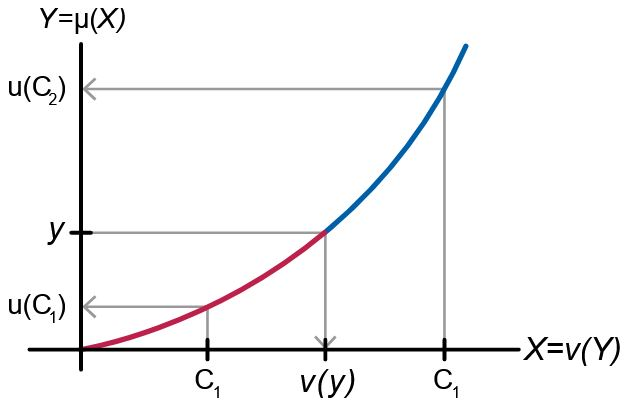
\includegraphics[scale=0.5]{CoVin.JPG}
    \caption{Graphical representation showing that all the inequalities hold}
\end{figure}

The blue curve represents the continuous and increasing function $Y=\mu(X)$ [$Y=g(X)$]. If $x$
values are inputted into the function then $y$ values $\mu(x)$ [$y$] are received. Since the function is \textbf{continuous}, \textbf{one-to-one} and
\textbf{increasing}, an inverse function $X=v(Y)$ [$X=g^{-1}(Y)$] where $y$ values are inputted then $x$
values $v(y)$ [$x$] are received.

The distribution of function $Y$ can be derived as:
\begin{align*}
    F_Y(y) = P(Y\leq y) = P[g(X) \leq g(x)] = P(X\leq x) = F_X (x)
\end{align*}

\begin{tcolorbox}[breakable,colback=white] 
    The PDF $f_Y(y)$ is the derivative of the CDF of $F_Y(y)$. 
    \begin{align*}
        f_Y(y) = F^\prime_Y (y) = f_X[v(y)]\: . \: v^\prime(y)
    \end{align*}
    or 
    \begin{align*}
        f_Y(y) = \frac{d\: F_X(x)}{dy} = \frac{d\: F_X (x)}{dx} \frac{dx}{dy} = f_X(x)\frac{dx}{dy}
    \end{align*}
\end{tcolorbox}

%%%%%%%%%%%%%%%%%%%%%%%%%%%%%%%%%%%%%%%%%%%%%%%%%%%%%%%%%%%%%%%%%%%%%%%%%%%%%%%%%%%%%%%%%%%%%%%%%%%%%%%%%%
\subsection{Generalisation for a decreasing function}

Let:
\begin{itemize}
    \item $X$ be a \textbf{continuous random variable}.
    \item $g(x)$ a strictly monotonic function (one-to-one function) defined over the support $c_1 < x < c_2$.
    \item $Y = g(X)$ be a continuous and decreasing function of $X$ with inverse function $X=g^{-1}(Y)$.
\end{itemize} 

\begin{figure} [h!]
    \centering
    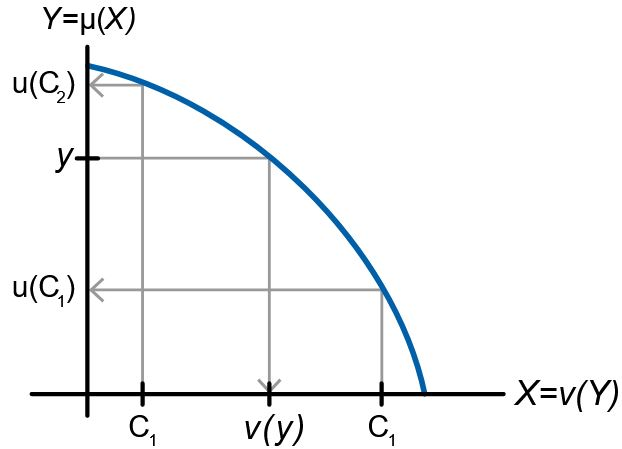
\includegraphics[scale=0.5]{CoVde.JPG}
    \caption{Graphical representation showing that all the inequalities hold}
\end{figure}

The distribution of function $Y$ can be derived as:
\begin{align*}
    F_Y(y) = P(Y\leq y) = P[g(X) \leq g(x)] = P(X\geq x) = 1 - F_X (x)
\end{align*}

\begin{tcolorbox}[breakable,colback=white] 
    The PDF $f_Y(y)$ is the derivative of the CDF of $F_Y(y)$. 
    \begin{align*}
        f_Y(y) = F^\prime_Y (y) = -f_X[v(y)]\: . \: v^\prime(y)
    \end{align*}
    or 
    \begin{align*}
        f_Y(y) = \frac{d\: F_X(x)}{dy} = \frac{d\: F_X (x)}{dx} \frac{dx}{dy} = - f_X(x)\frac{dx}{dy}
    \end{align*}
\end{tcolorbox}

%%%%%%%%%%%%%%%%%%%%%%%%%%%%%%%%%%%%%%%%%%%%%%%%%%%%%%%%%%%%%%%%%%%%%%%%%%%%%%%%%%%%%%%%%%%%%%%%%%%%%%%%%%
\end{document} 